\chapter{State of the Art}
\label{State of the Art}
\thispagestyle{empty}



The objective of this chapter is to go into detail about key aspects of reinforcement learning, the core topic of this thesis. In particular, we will describe the concept of Decision Markov Process, the experiment environment, the concept of state, actions, and reward function. Eventually, we will give insight about the algorithms we used in this project: Fitted Q-Iteration, and Deep Deterministic Policy Gradient. 
Then, in the following section, we will show some successful application on reinforcement learning to autonomous driving, videogames, and in particular racing games.


\section{Theoretical Background}

\subsection{Reinforcement Learning}
Together with Supervised Learning and Unsupervised Learning, Reinforcement Learning is a branch of Machine Learning, the discipline which studies the way a computer program can learn from experience and improve its performance at a specified task. Whereas Supervised Learning algorithms are based on inductiove inference where the model is tipically trained using labelled data to perform classification or regression, and Unsupervised Learning exploits techniques of density estimation and clustering applied to unlabelled data, in the Reinforcement Learning paradigm an autonomous agent learns to improve its performance at an assigned task by interacting with its environment.
Tipically, Reinforcement Learning agents are not explicitly taught how to act by an expert. Instead, the agent is free to explore the environment in which it lives, and its performance is evaluated by a reward function. Its goal is to maximize the reward by acting accordingly. The resulting reward results from the sum of the reward gained at every single step in its exploration process: for each state, the agent chooses an action to take and receives a reward based on the usefulness of its decision. Eventually, the agent learns the way to obtain the highest reward by exploiting knowledge learned about the expected utility of different state-action pairs. The challenge of Reinforcement Learning is to design the best tradeoff between exploration and exploitation, that is the capability of an agent of use its knowledge to obtain high rewards and, by contrast, being capable of exploring new possibilities in such a way not to remain stuck in a local optimum. Intuitively, the exploration process is high at the first iterations of the learning process, while it should decrease with accumulating knowledge.

\subsubsection{Markov Decision Process}
The Reinforcement Learning problem can be formalized as a Markov Decision Process. A MDP is a tuple composed by:
\begin{itemize}
  \item A finite set of states \(D\): it encompasses every possible state of the process
  \item A finite set of actions \(A\): it represents the possible action the agent can take at any moment
  	\item A reward function \(r = \psi(s_t,a_t,s_{t+1})\), which represents the reward given to the agent at state \(s_t\) taking the action \(a_t\) landing in the state \(s_{t+1}\)
  	\item A transition probability model \(T(s_t,a_t,s_{t+1}) = p(s_{t+1}|s_t,a_t)\), which indicates the probability of landing in a state \(s_{t+1}\) being in a state \(s_t\) taking an action \(a_t\)
\end{itemize}

This provides the framework in which Reinforcement Learning operates: its goal is to find a policy \(\pi\) which specifies the actions to take in each state in order to maximize the reward over time i.e. fulfill the task.
Reinforcement learning can solve Markov decision processes without explicit specification of the transition probabilities; the values of the transition probabilities are needed in value and policy iteration. In reinforcement learning, instead of explicit specification of the transition probabilities, the transition probabilities are accessed through a simulator that is typically restarted many times from a uniformly random initial state. Reinforcement learning can also be combined with function approximation to address problems with a very large number of states.
Reinforcement Learning operates under the Markov Assumption, under which the current state represents all the information needed to take an action, regardless from the past states and actions.
In other words: "The future is independent of the past given the present"

\subsubsection{Environment}
The environment is the mathematical representation of the world in which the agent operates. It reflects the set of features of a machine learning problem, which could be numerical (such as e.g. coordinates, velocities, acceleration) or raw (such as images or signals). On the representation of the environment depends the choice of the algorithm suitable to perform a learning process.

\subsubsection{Reward}
At each timestep, the agent receives a reward by the reinforcement learning algorithm, accordingly to the usefulness of action taken.
At the end of an episode (a finite sequence of states) the return is tipically computed as \[R_t = \sum^{T}_{k=0}\gamma^k r_t + k +1\] where \(\gamma\) represents a discount factor comprised between 0 and 1, which stands for a learning paramenter that influences how the agent considers future                              or present reward. A small \(\gamma\) results in a higher consideration of present rewards than the future (often caled "myopic" evaluation), while with a \(\gamma\) near to 1, the agent will consider equally the reward coming from the present either from the future (also called "far-sighted" evaluation). The role of the discount factor resides in the fact that, besides being mathematically convenient, it avoids infinite returns in cyclic Markov Process, and it's capable of addressing a non-fully represented uncertainty about the future.

\subsubsection{Policy}
The goal of reinforcement learning is finding a policy \(\pi\), which maps states to a probability distribution over the actions, in order to maximize the return. This policy is called optimal policy \(\pi^*\).
If from a state \(s_t\) the agent takes always the same action \(a_t\), the policy is deterministic:
\(\pi(s_t) = a_t\)
Otherwise, if the taking of an action rather than another is due to a probability distribution, the policy is called stochastic:
\(\pi(a_t|s_t) = p_i, 0<=p_i<=1\)

\subsection{Policy Evaluation}
In order to evaluate the usefulness of a policy, we now introduce the concept of Value Function, which is computed as the discounted sum of rewards as discussed before in the return.


\[V^\pi(s) = \mathbb{E}_\pi{\left[R_t|s_t=s\right]}= \mathbb{E}_\pi\left[\sum^{\infty}_{i=0}\gamma^ir_{t+i+1|s_t=s}\right] = \mathbb{E}_\pi\left[r_{t+1} + \sum^{\infty}_{i=0}\gamma^ir_{t+i+2|s_t=s}\right]\]
. . . finire


Parallel to the value functions is the concept of action-value function, or Q-value, which is the expected return after taking an action \(a_t\) in state \(s_t\) and thereafter following policy \(\pi\):
\[Q^\pi(s_t,a_t)=\mathbb{E}_{r_{i \geq t},s_{i>t} \sim ,a_{i>t} \sim \pi}[R_t|s_t,a_t]\]
from which can be derived the recursive form the Bellman Equation:
\[Q^\pi(s_t,a_t)=\mathbb{E}_{r_t,s_{t+1} \sim E }\left[ r(s_t,a_t) + \gamma \mathbb{E}_{a_{t+1} \sim \pi}\left[Q^\pi (s_{t+1},a_{t+1})\right]\right]\]


\subsection{Temporal Difference Learning}
\subsubsection{SARSA}

\subsubsection{Q-Learning}
\subsubsection{Issues with Temporal Difference Learning}
\subsection{Deep Reinforcement Learning}

\subsubsection{Actor-Critic Methods}
The "Critic" estimates the value function. This could be the action-value (the Q value) or state-value (the V value).
The "Actor" updates the policy distribution in the direction suggested by the Critic (such as with policy gradients).
and both the Critic and Actor functions are parameterized with neural networks. In the derivation above, the Critic neural network parameterizes the Q value - so, it is called Q Actor Critic.
\subsubsection{Fitted Q-Iteration}

\subsubsection{Deep Deterministic Policy Gradient}
It is not possible to straightforwardly apply Q-learning to continuous action spaces, because in continuous spaces finding the greedy policy requires an optimization of a t at every timestep; this opti-
mization is too slow to be practical with large, unconstrained function approximators and nontrivial action spaces. Instead, here we used an actor-critic approach based on the DPG algorithm.





















- FQI

	When the state and action spaces are finite and small enough, the Q-function can be represented in tabular form, and its approximation (in batch and in on-line mode) as well as the control policy derivation are straightforward. However, when dealing with continuous or very large discrete state and/or action spaces, the Q-function cannot be represented anymore by a table with one entry for each state-action pair. Moreover, in the context of reinforcement learning an approximation of the Q-function all over the state-action space must be determined from finite and generally very sparse sets of four-tuples.
To overcome this generalization problem, a particularly attractive framework is the one used by Ormoneit and Sen (2002) which applies the idea of fitted value iteration (Gordon, 1999) to kernel-based reinforcement learning, and reformulates the Q-function determination problem as a sequence of kernel-based regression problems. Actually, this framework makes it possible to take full advantage in the context of reinforcement learning of the generalization capabilities of any regression algorithm, and this contrary to stochastic approximation algorithms (Sutton, 1988; Tsitsiklis, 1994) which can only use parametric function approximators (for example, linear combinations of feature vectors or neural networks). In the rest of this paper we will call this framework the fitted Q iteration
algorithm so as to stress the fact that it allows to fit (using a set of four-tuples) any (parametric or non-parametric) approximation architecture to the Q-function.
The fitted Q iteration algorithm is a batch mode reinforcement learning algorithm which yields an approximation of the Q-function corresponding to an infinite horizon optimal control problem with discounted rewards, by iteratively extending the optimization horizon (Ernst et al., 2003).
At each step this algorithm may use the full set of four-tuples gathered from observation of the system together with the function computed at the previous step to determine a new training set which is used by a supervised learning (regression) method to compute the next function of the sequence. It produces a sequence of Q N -functions, approximations of the Q N -functions defined by Eqn (5). --> mettere algoritmo a pag 6 di tree based batch reinforcement learning

- extra trees
	Besides Tree Bagging, several other methods to build tree ensembles have been proposed that often improve the accuracy with respect to Tree Bagging (e.g. Random Forests, Breiman, 2001). In this paper, we evaluate our recently developed algorithm that we call "Extra-Trees", for extremely randomized trees (Geurts et al., 2004). Like Tree Bagging, this algorithm works by building several (M) trees. However, contrary to Tree Bagging which uses the standard CART algorithm to derive the trees from a bootstrap sample, in the case of Extra-Trees, each tree is built from the complete original training set. To determine a test at a node, this algorithm selects K cut-directions at random and for each cut-direction, a cut-point at random. It then computes a score for each of the K tests and
chooses among these K tests the one that maximizes the score. Again, the algorithm stops splitting a node when the number of elements in this node is less than a parameter n min . Three parameters are associated to this algorithm: the number M of trees to build, the number K of candidate tests at each node and the minimal leaf size n min . The detailed tree building procedure is given in Appendix A.
	
	- Double learning
	- Double FQI

- DDPG
	- DPG
	



- background:
pag 3-4 cinesi



Presented in [16], Deep Q-learning from Demonstrations
(DQfD) vastly accelerates DQN by pretraining an initial
behavior network, and also introducing a supervised loss and
a L2 regularization loss when training the target network.

A combination of the advantages of both, the speed of the Riccati controller and the generality of MPC, can be achieved by finding a function that maps state values to
control variables, e. g., by training a deep neural network. Such a model could, for example, be learned supervised, as done for PILOTNET, or by reinforcement learning. The latter in particular led to excellent results in the training of such agents for controlling real-world systems such as robots or helicopters.
Recent work also shows promising applications of reinforcement learning for autonomous driving by making strategic decisions. 
Autonomous driving tasks where RL could be applied include: controller optimization, path planning and trajectory optimization, motion planning and dynamic path planning, development of high-level driving policies for complex navigation tasks, scenario-based policy learning for highways, intersections, merges and splits, reward learning with inverse reinforcement learning from expert data for intent prediction for traffic actors such as pedestrian, vehicles and finally learning of policies that ensures safety and perform risk estimation. Further, it turns out to be suitable in contexts of autonomous racing: the driverless racer could learn a policy that is able to outperform the performance of a human driver, or a policy taught by experts.





\section{Related Works}



In this section we'll describe some of the applications of Reinforcement Learning in the context of videogames, autonomous driving and racing. 


\subsection{Reinforcement Learning in Videogames}

All the Reinforcement Learning algorithms require interaction with the environment to learn a policy the gathered experience. Trajectories can be collected by using real world environment or through a simulator. 
Both approaches have pros and cons, and the choice mainly depends on the context and the application of the learning agent. 
A simulator is preferred when the exploration is not dangerous, whereas simulator when the real agent can hurt itself or damage environment. 
The drawbacks of learning in a physical system reside mainly in the fact that exploration may be dangerous, and learning is expensive. A learning agent is often a robot, composed of mechanical parts, which may perform a range of movements that can be harmful - to itself, to other people, to the environment itself - if not behaving in an intended manner. Think about a car hitting a wall, and with a person aboard. Simulators, on the other hand, are safe: everything is happening inside a computer, in a virtual world, and every - or almost - can be properly tuned before putting the code on the physical robot. Another downside of learning in the real world is expensiveness: machine learning, relying on statistics, requires vast amount of data to be available, which in a RL context translates in a big number of repetition of an experiment. In a physical environment the components are typically more expensive than on a simulator, which requires AC current to power one or more machines. A robot requires one or more engines, which can be electrical (consuming much more than computers) or combustion-like, which require some kind of fuel, like gasoline. Moreover, wears comes into play, which requires fixing, or replacing, for instance the wear of tyres due by friction with asphalt. Finally, possibles repaires required when the robot crashes or hurts itself of the environment must be taken into account
On the contrary, in the real world there is model-free, thus, the learning outcome is typically more accurate than on simulator, or better, it doesn't need aposteriori fine-tunings, which may be need to be taken into account when learning in a simulation environment. In fact, whether simulators may be preferred for the reasons listed above, they have drawbacks, too.
A simulated environment must replicate the world and an agent to a certain degree of accuracy: replicating a perfect copy would be unfeasible, because of the power of computation required to run it, and the intrinsic complexity of the rules which govern it, which today are known to a certain extent. On the other side, a simple representation of the world is much more lean to run, and simple to be coded, but may be undermodeling with respect to the task. The main difficulty here is finding is the best trade off. Another aspect to take into consideration when choosing to learn on a simulated environment is that the computed parameters of the equations ruling the world and the actions to fulfill a task may be different to the real ones, thus may need some fine tuning when embodied into the machine. This is due to all the aspects which are not taken into account by the model of the simulator. For instance, wear of components and deformation dynamics are ruled by complex models which are hard to replicate on simulators.
As said, the choice between real environment and a simulated one mainly depends on the context and the application of the learning agent. When exploration is not dangerous, real world environments are preferred whereas simulator when the real agent can hurt itself or damage environment.
Thanks to the flexibility of the reinforcement learning algorithms, which enable an agent to learn a behavior from its experience, by giving a representation of the world a which don't require an apriori knowledge of its dynamics, reinforcement learning is particularly suitable to the contexts which permit to perform many tries of a particular task. For this reason, videogames and computer simulators are adapt to run a reinforcement learning algorithm on.
A notorius videogame played by a RL autonomous agent is Atari \cite{atari} by Google's Deepmind. By learning a deep convolutional neural network to approximate the Q-function, Mnih et al. successfully construct a Deep Reinforcement Learning framework called Deep Q-Network (DQN) which plays Atari games in human level. It takes as representation of the world the raw pixels and learns an end-to-end policy which maximizes the q-values.
Another famous example is Alphago also by Deepmind \cite{alphago}, which beated for several years consecutively the human champion at Go game. This is not a videogame but a board game, but the case is noteworthy, because such game is known for being one of the most complex  for his huge set of rules, which makes brute-force approaches infeasible. To achieve this result, it has been trained with a supervised learning neural network from past experience, and then, a reinforcement learning algorithms has been applied to try and beat itself's own play. 
In racing games, which is the scope of our thesis, different solutions has been proposed over the years. In the next section we'll introduce the concept of autonomous driving and in particular in the racing context. We'll expose the problem of finding the optimal trajectory and explore some of the state-of-the-art-techniques which tackle this issue.


\subsection{Autonomous Driving in Videogames}
Finding a racing line that allows to achieve a competitive lap-time is a key problem in real-world car racing as well as in the development of non-player characters for a commercial racing game.
The optimal racing line is defined as the line to follow to achieve the best lap-time possible on a given track with a given car. The optimal racing line is the path that a driver should follow to complete a lap on a given track in the smallest amount of time possible. As the lap-time depends both on the distance raced and on the average racing speed, finding the optimal racing involves two different sub-problems: racing the shortest distance possible and racing as fast as possible along the track.

Over the years, different attempts to achieve time-optimal racing, evolving together with technology. Besides Reinforcement Learning, controlling a self-driving car can be done with a planner, if the optimal trajectory is a priori computed, or by a controller. In this section, we provide an overview of such techniques. 


Botta et al. \cite{botta} show how to encode a racing line by a set of connected B\'{e}zier curves, such that each gene defines a small portion of the racing line. B\'{e}zier curves are a family of parametrized curves widely used in computer graphics and in related fields. Initially used for drawing cars, nowadays B\'{e}zier curves are frequently used in vector graphics to model smooth paths, as they offer a compact and convenient representation.
A B\'{e}zier curve is defined by a set of control points, with the first and the last one being respectively the beginning and the end of the curve, while the intermediate control points do not usually lie on it. Therefore, the evolution is responsible of the entire design of the racing line.  
  \begin{figure}
    \centering
 	  \captionsetup{width=10cm}
      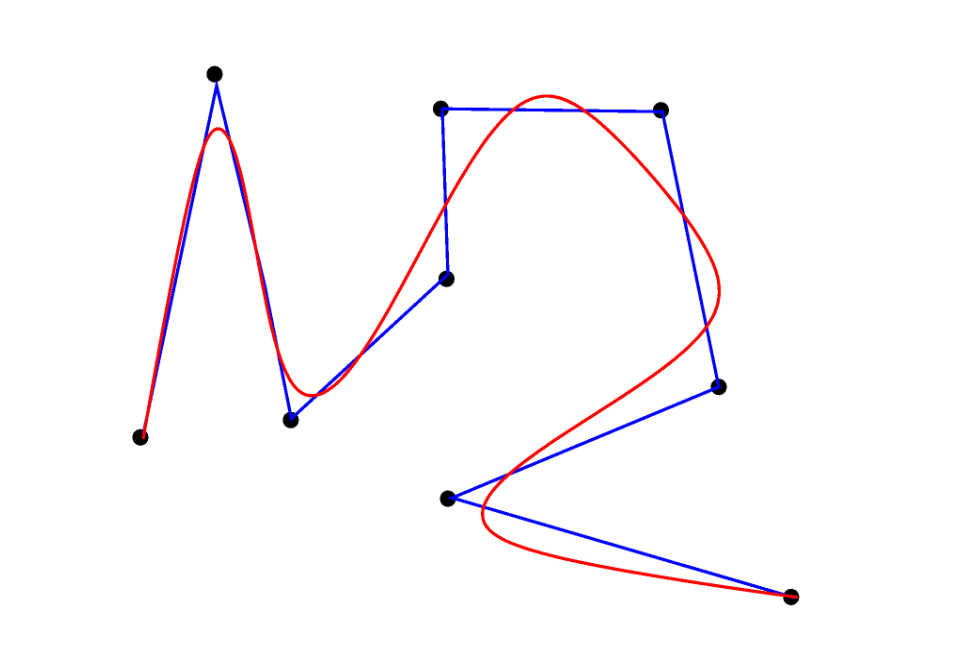
\includegraphics[width=10cm]{./img/bezier}
     \caption{From \cite{botta}. An example of B\'{e}zier curve: black points are the control point of the curve; blue lines simply connect with straight segments the control points; red line is the resulting B\'{e}zier curve.}
  \end{figure}
In addition, the authors compare two different methods to evaluate the evolved racing line; the first one is based on testing the evolved racing lines in a racing simulator; the second one consists of estimating the performance of a racing line through a computational model.
The former consists in making a TORCS predefined controller follow a determined trajectory. Then, a fitness function is computed as the lap-time achieved during the best lap. While this approach does not require any previous domain knowledge, as the fitness is the result of simulation, it is also rather expensive in computational terms as it requires a full simulation. 
On the contrary, the latter relies on a computational model which provides an estimate of the lap-time
that could be achieved following the racing line to evaluate. In particular, as soon as an estimate of the lap-time is available, the fitness function is computed as in the simulation-based method. This way, the computation is generally significantly less expensive than the simulation-based evaluation. As a drawback, a previous domain knowledge is required in order to estimate the speed that can be reached in each point of the racing line, such as car dynamics and the track grip. Moreover, the accuracy of the estimation depends on the precision of the model itself.

Another approach has been proposed by Bonyadi et al: in \cite{ahura} they implemented a controller called Ahura for TORCS based on heuristics.
The controller uses five modules: 
\begin{itemize}
\item Steer controller: This module uses the estimated angle
of the turn in front and the vacant distance in front to determine the steer angle. The module can control how smooth or sharp the vehicle is going to turn.
The main idea behind calculation of the steer angle is to find the proximity sensor that has the maximum empty space in front (called the base sensor). The angle of the base sensor, together with some other auxiliary proximity sensors, is then used to set the angle of the steer.
\begin{figure}
 \centering
  \captionsetup{width=10cm}
  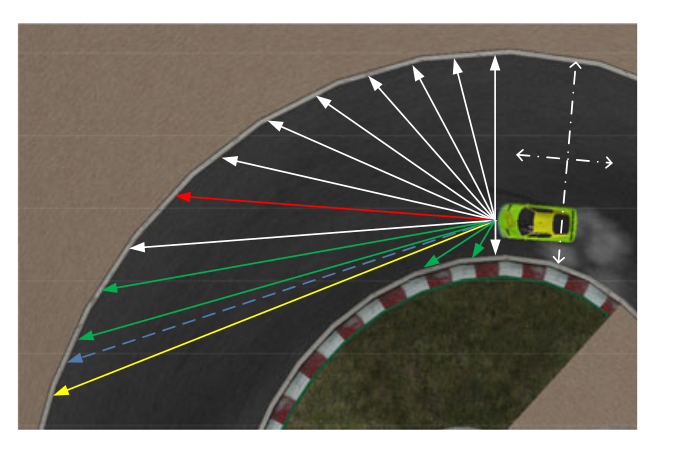
\includegraphics[width=10cm]{./img/ahura-steer}
  \caption{From \cite{ahura}. Red vector, the yellow vector, green vectors, and the blue vector represent the zero sensor, the base sensor, auxiliary sensors, and the final angle to take the turn, respectively.}
\end{figure}
\item Speed controller: The aim of the speed controller is to determine the speed that the vehicle can move according to the current situation without considering opponents. This decision then is translated to the acceleration/breaking pedals. This module uses the estimated turn angle together with the vacant distance in front to decide the safe speed.
The target speed is mapped with a nonlinear function to values of acceleration and brake. Then, it is necessary to make sure that these values are applied in an appropriate way.  During the brake, the spin of thewheels might become smaller than the speed of the vehicle that
means the wheels are slipping. Also, during the acceleration, the spin of the wheels might increase more than the speed of the vehicle that means the vehicle is in traction. The ABS and ASR technologies solve these issues through keeping the speed of the spinning wheels and the speedof vehicle as close as possible.
Moreover, a gearing system is implemented, based based on the minimum and maximum values of the rpm for each gear.
\item Opponent manager: This module creates a map of oppoents around and finds the vacant slot to overtake. This action may entail modification of the speed and steer calculated by the speed and steer controller modules.
Ahura’s opponent manager contains two modules, steer reviser and speed reviser, that are responsible to revise steer and speed for overtaking. The information about opponents provided by opp sensors contain their distance and angle from the current position of the vehicle. This means that the position of opponents is provided in a polar coordinates system with the center of the measuring vehicle. Ahura builds a spatial map of the position of opponents based on the information provided by the opp sensors. This map is used to revise steer and speed of the vehicle for overtaking purposes.
\item Dynamic adjuster: This module uses the mechanical specifications of the track (friction, bumps) as well as recorded difficulties the controller has experienced during the earlier laps and adjusts the current driving style.
The dynamics parameters are estimated using an optimization-based approach to find the best values so that Ahura can drive a specific bot in TORCS. There are 23 parameters in Ahura that need to be determined: eight parameters for the steer controller, ten parameters for the speed controller, five parameters for the opponent manager.
They were determined by using the optimization algorithm CMA-ES \cite{cmaes}, which has a good performance in continuous space, works with nonlinear systems, no constraint handling technique is required, and it is appropriate for nonseparable search spaces.
\item Stuck manager: This module controls the vehicle when it is out of the track or it has stuck somewhere.
The calculated parameters for the speed and steer controllers need to be revised based on the specifications of the track. The reason is that the parameters have been set for a limited number of tracks while new tracks might have different specifications. The main characteristics of tracks that may affect the best choice for parameters are friction, width, and bumps. Also, Ahura is able to handle stuck situation. In fact, if Ahura recognizes that it is off the track, it reduces the maximum value of the acceleration pedal to prevent too much traction. It finds the correct direction first and tries to get back to the track. If it detects that the car is not moving, the gear is changed to -1 (rear gear) and the steer is adjusted accordingly to repair the direction of movement.
\end{itemize}


Existing advanced control based attempts to minimum-time driving usually provide only offline open-loop solutions.
In \cite{mpc}, the authors experimentally compared different time-optimal nonlinear MPC \cite{mpc_orig} formulations based on least squares objectives with an economic cost function in a real-time setup of small-scale model race cars, with the help of ACADO simulation toolkit from MATLAB \cite{acado}.
MPC, standing for Model Predictive Control is a multivariable control algorithm that uses an internal dynamic model of the process, a cost function over the receding horizon and an optimization algorithm minimizing the cost function using the control input.
The tight real-time bounds imposed on computational times make it necessary to reformulate the problem so as to allow for the use of efficient algorithms. To this end, they employed a nonlinear bicycle model \cite{bycicle} in a reformulation to spatial coordinates and proposed an infeasible-time-tracking objective for the best practical results.
For an approximate solution of the time-optimal driving problem, the aim is to minimize the time required for the race car to reach the end of the fixed-length spatial prediction horizon. For prediction horizons which tend to infinity, this objective tends to the goal of driving time-optimally. As a consequence, long horizons are expected to yield a good approximation of the original problem in practice.
In the author's formulation, by providing a suffciently small (i.e., infeasible) "target time" T ref they can have an approximate time-
optimal MPC formulation in least-squares form. 
The real-world experiments showed that this approach has potential, but the bicycle model proved insufficient at high velocities due to slip effects not being modelled.
\begin{figure}
 \centering
  \captionsetup{width=10cm}
  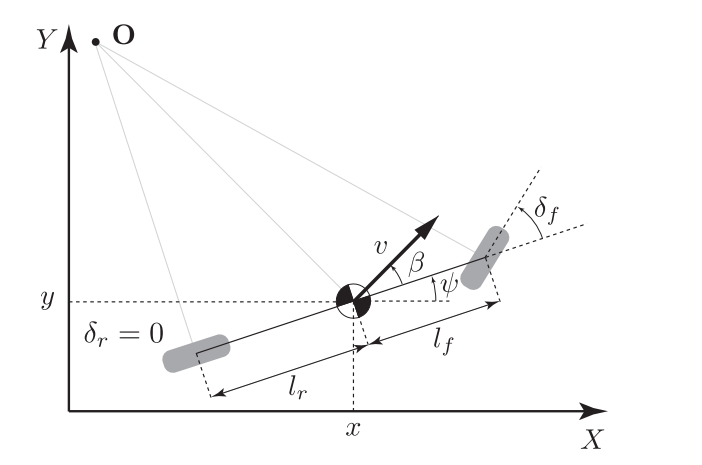
\includegraphics[width=10cm]{./img/bycicle}
  \caption{From \cite{mpc}. Kinematic Bicycle Model}
\end{figure}
\begin{figure}
 \centering
  \captionsetup{width=10cm}
  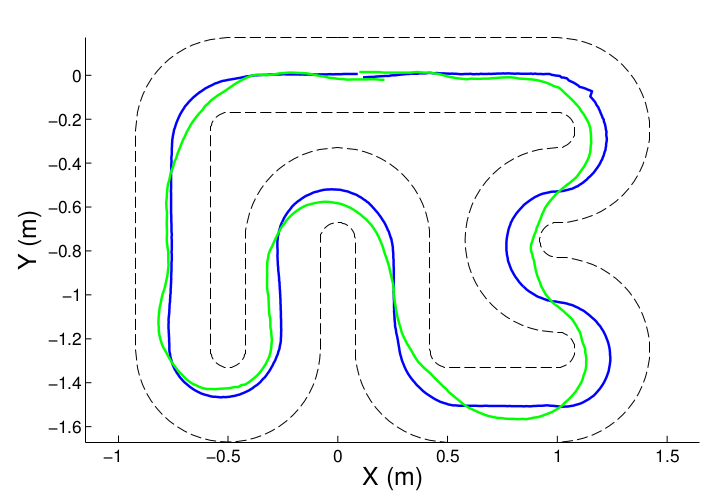
\includegraphics[width=10cm]{./img/mpc-comparison}
  \caption{From \cite{mpc}. Comparison of the performance of trajectory tracking and time-optimal driving on the experimental setup.}
\end{figure}

\subsection{Reinforcement Learning in Racing Videogames}

With the evolving of technologies and algorithms, the focus has been shifting towards reinforcement learning and in general data-driven algorithms, that has been proven to outperform classical algorithms in a variety of applications, including autonomous driving and racing.

Due to the complexity of the problem, the most successful approaches has been proved to be the ones that incorporate an automatic learning process with human expertise.

In \cite{cardamone} Cardamone, Loiacono and Lanzi applied supervised learning to develop car controllers for The Open Car Race Simulator from the logs collected from other drivers. 
They considered two representations of the current state of the car: the set of rangefinder inputs usually employed in simulated car racing competitions, and a high-level, qualitative, representation involving basic lookahead information about the track in front of the car. Instead of predicting the typical low-level actions on the car actuators available in TORCS (namely, the steering wheel, the gas pedal, the brake pedal and the gear change), their approach predicts a target speed and the car position with respect to the track axis.
They considered two supervised learning methods, multi-layer neural networks and k-nearest neighbor classifiers, and applied them to compute a model mapping input sensors to actions which could imitate the behavior of an observed driver.

In \cite{cinesi} the authors addresses an issue which is similar to ours: they aim at integrate a reinforcement learning algorithm with human expertise. Their claim is that this process could help accelerate the exploration phase and increase learning agent's stability.
Their framework is a continuous reinforcement learning setting, in which they integrate DDPG with human demonstrations.
To achieve that, they formulate a loss function to optimize which combines the experience gathered from the environment and by the demonstrations. In such a way, with respect to a state, the agent should pick an action wich is consisent with the human behavior.

 Our work proposed different approaches to solve time-optimal racing problem in the framework of reinforcement learning. ampliare, parlare di torcs
 
 
 
 

-expertise
-loiacono
-cinesi